%! TEX root = ../am2-20-21.tex

\chapter{Integrale triple}
\index{integrale!triple}

Integralele triple pe care le vom calcula se rezolvă folosind o abordare
de tipul domeniilor intergrafic. Astfel, dacă $ \Omega $ este un domeniu de tip
corp tridimensional, delimitat de suprafețe de ecuații date, se poate calcula
\emph{volumul} domeniului $ \Omega $ cu formula:
\[
    V(\Omega) = \iiint_\Omega dxdydz,
\]
iar de cele mai multe ori, se calculează inițial integrala după $ z $, deoarece
suprafețele sînt date în această formă.

\vspace{0.5cm}

\textbf{Exercițiu:} Calculați volumul corpului delimitat de suprafețele
de ecuații date:
\begin{enumerate}[(a)]
    \item $ z = x^2 + y^2 $ (paraboloid) și $ z = x + y $ (plan);
    \item $ z = x^2 + y^2 - 1 $ și $ z = 2 - x^2 - y^2 $ (2 paraboloizi);
    \item $ x^2 + y^2 + z^2 = 1 $ (sferă) și $ x^2 + y^2 = \dfrac{1}{2} $ (cilindru).
\end{enumerate}

Indicații: (a) Se calculează mai întîi integrala după $ z $, deoarece o reprezentare
grafică ne va ajuta să vedem că în sensul crescător al axei $ OZ $ întîlnim
mai întîi paraboloidul, apoi planul, conform figurii \ref{fig:plan-parab}.

\begin{figure}[!htbp]
    \centering
    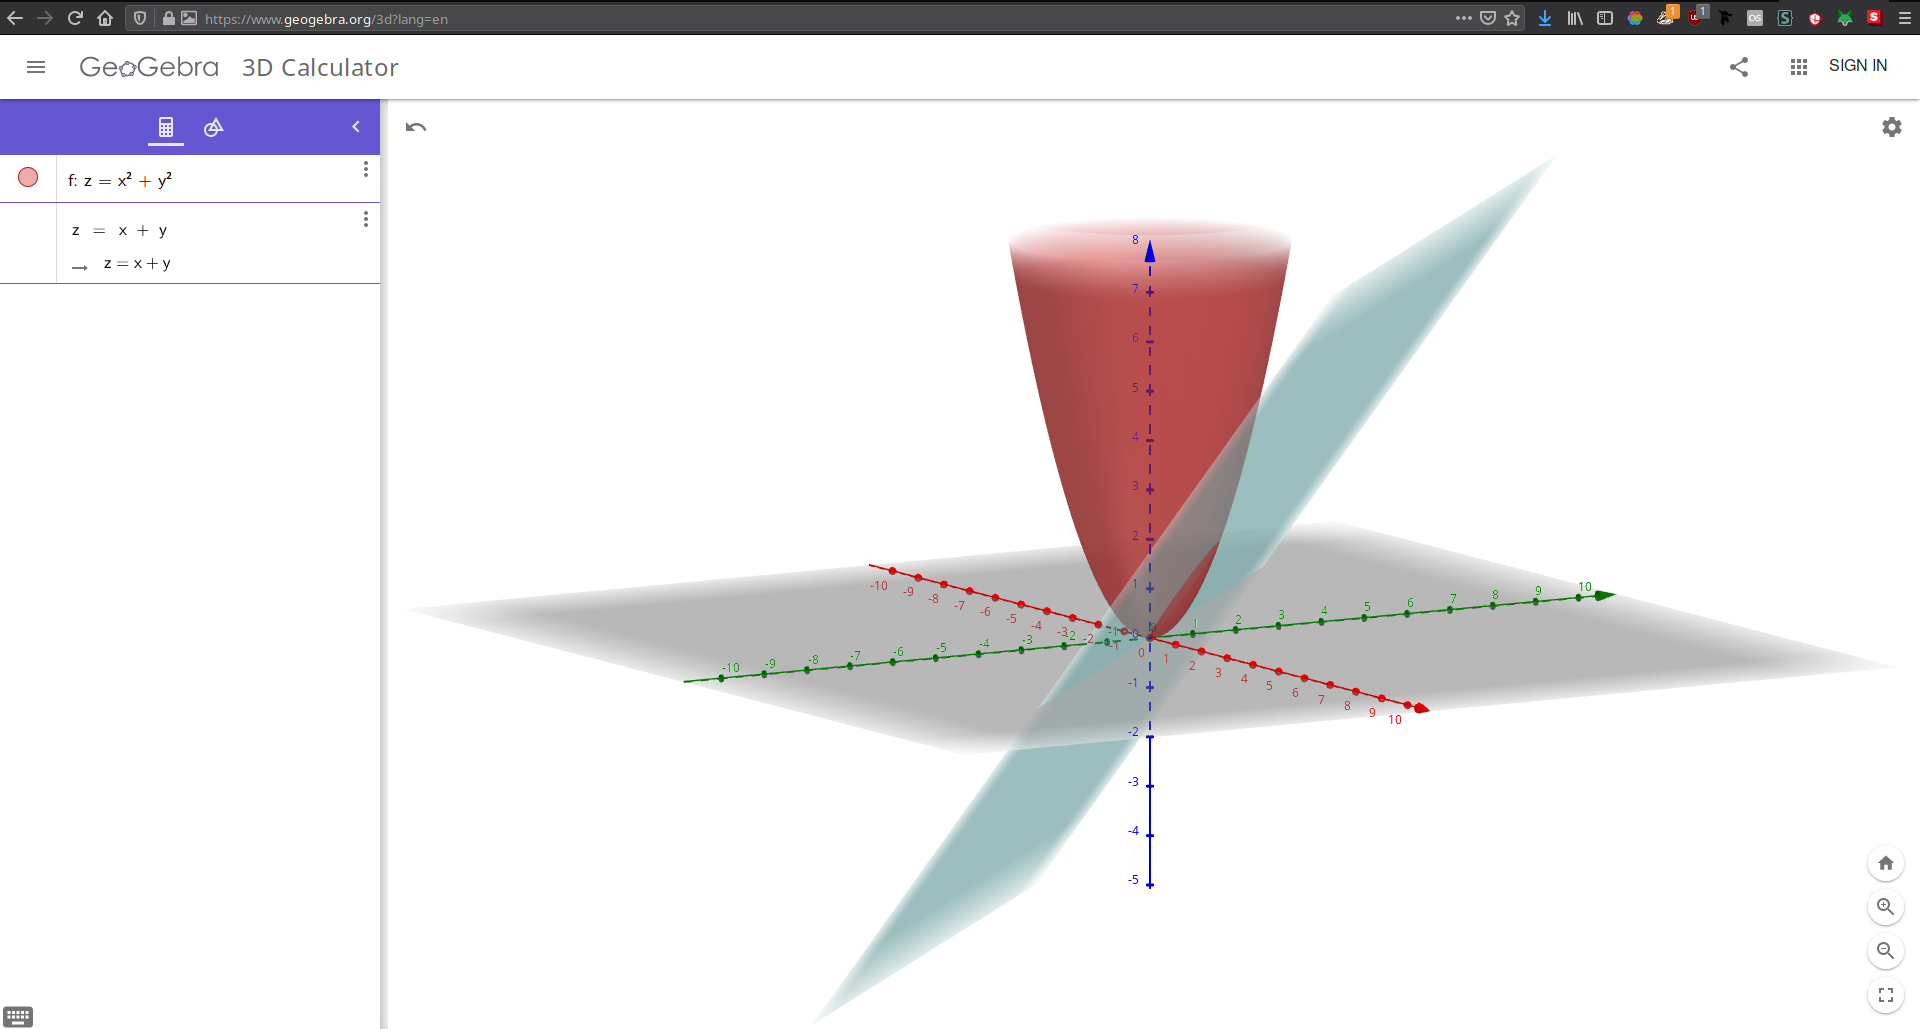
\includegraphics[scale=0.2]{fig/plan-paraboloid.png}
    \caption{Intersecția între paraboloidul $ z = x^2 + y^2 $ și %
    planul $ z = x + y $}
    \label{fig:plan-parab}
\end{figure}

Astfel, avem de calculat:
\[
    V(\Omega) = \iiint_\Omega dxdydz = \iint_D \int_{x + y}^{x^2 + y^2} dz dx dy,
\]
unde $ D $ este proiecția pe planul $ XOY $ a figurii, care se poate obține
foarte simplu eliminînd $ z $ din cele două ecuații, adică:
\[
      x^2 + y^2 = x + y,
\]
care este un cerc. După aceea, integrala pe $ D $ se calculează ca o integrală
dublă.

\vspace{0.5cm}

\textbf{Atenție!} Volumul unui corp, ca și aria unui domeniu bidimensional,
trebuie să fie pozitiv! Dacă din calcule corecte rezultă un volum negativ,
înseamnă că s-au luat greșit capetele de integrare (în exemplul de mai sus
s-a luat $ z $ de la paraboloid la plan).

\vspace{0.5cm}

În unele exerciții, în special cînd apar sfere sau cilindri, se pot folosi
coordonate specifice:

\textbf{Coordonatele sferice:} 
$ (r, \theta, \varphi) \in \RR_+ \times [0, \pi) \times [0, 2\pi) $, reprezentate
în figura \ref{fig:coord-sph}.

\begin{figure}[!htbp]
    \centering
    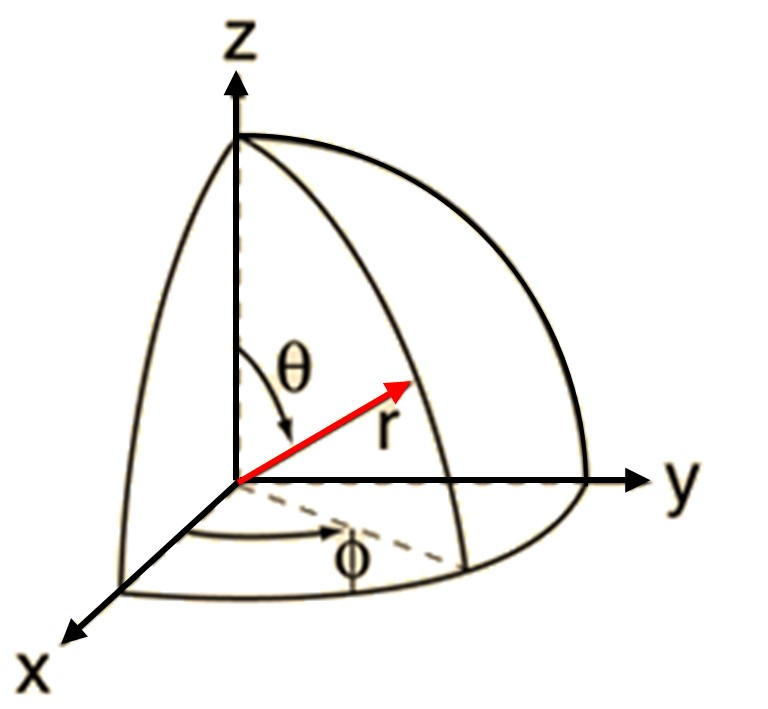
\includegraphics[scale=0.25]{fig/coord-sph.jpg}
    \caption{Coordonatele sferice $ r, \theta, \varphi $}
    \label{fig:coord-sph}
\end{figure}

Schimbare de coordonate este dată de:
\[
    \begin{cases}
        x &= r \sin \theta \cos \varphi \\
        y &= r \sin \theta \sin \varphi \\
        z &= r \cos \theta
    \end{cases}.
\]

Nu uitați, în acest caz, să calculați și jacobianul schimbării de coordonate:
\[
    J = \begin{vmatrix}
            x_r & x_\theta & x_\varphi \\
            y_r & y_\theta & y_\varphi \\
            z_r & z_\theta & z_\varphi
        \end{vmatrix}.
\]

\textbf{Coordonate cilindrice:} $ (r, t, z) \in \RR_+ \times [0, 2\pi) \times \RR $,
care sînt, practic, coordonatele polare, \qq{mutate} în lungul axei $ OZ $.
De aceea, schimbarea de coordonate este dată de:
\[
    \begin{cases}
        x &= r \cos t \\
        y &= r \sin t \\
        z &= z
    \end{cases}.
\]

Iar jacobianul transformării se calculează similar, cu derivatele lui $ x, y, z $
în raport cu $ r, t $ și respectiv $ z $.
\index{coordonate!sferice}
\index{coordonate!cilindrice}

%%%%%%%%%%%%%%%%%%%%%%%%%%%%%%%%%%%%%%%%%%%%%%%%%%%%%%%%%%%%%%%%%%%%%%
\section{Exerciții suplimentare}

Calculați volumul corpurilor delimitate de suprafețele de ecuații:

\begin{enumerate}[(a)]
    \item $ x^2 + y^2 + z^2 = 8 $ și $ x^2 + y^2 - 2z = 0 $;
    \item $ z = 4 - x^2 - y^2 $ și $ 2z = 5 + x^2 + y^2 $;
    \item $ 2x^2 + y^2 + z^2 = 1 $ și $ 2x^2 + y^2 = z^2 $, pentru $ z \geq 0 $;
    \item $ x^2 + y^2 = 1 $ și $ z^2 = x^2 + y^2 $, pentru $ z \geq 0 $.
\end{enumerate}



%%%%%%%%%%%%%%%%%%%%%%%%%%%%%%%%%%%%%%%%%%%%%%%%%%%%%%%%%%%%%%%%%%%%%%
\section{Resurse suplimentare}

\begin{itemize}
    \item Lecțiile online ale Prof.\ Travis Kowalski, în special lista
        \texttt{Calculus 3}, începînd cu lecția 17 pentru integrale duble:
        \href{https://www.youtube.com/watch?v=le1JlwBkAog&list=PLE7F8F33E161D1425&index=23}{link};
    \item \texttt{GeoGebra}, pentru reprezentări grafice, în special
        tridimensionale: \href{https://www.geogebra.org/3d?lang=en}{link};
    \item Exerciții rezolvate ale Prof.\ R.\ Purtan de la ETTI:
        \href{https://adrianmanea.xyz/docs/18-19-etti-am1/purtan-int-duble.pdf}{integrale duble}
        și \href{https://adrianmanea.xyz/docs/18-19-etti-am1/purtan-int-triple.pdf}{integrale triple}.
\end{itemize}
